\section{Glass Moir\'e Patterns}
\label{sec:glass_patterns}

When a random dot pattern is scaled, rotated, and superimposed over
the original dots, interesting visual patterns known as Glass Patterns
emerge\footnote{L. Glass. 'Moir\'e effect from random dots' Nature 223,
  578580 (1969).}  In this exercise, we generate random dot fields
using numpy's uniform distribution function, and apply
transformations to the random dot field using a scale $\mathbf{S}$
and rotation $\mathbf{R}$ matrix $\mathbf{X_2} = \mathbf{S} \mathbf{R}
\mathbf{X_1}$.

If the scale and rotation factors are small, the transformation is
analogous to a single step in the numerical solution of a 2D ODE, and
the plot of both $\mathbf{X_1}$ and $\mathbf{X_2}$ will reveal the
structure of the vecotr field flow around the fixed point (the
invariant under the transformation); see for example the
\textit{stable focus}, aka \textit{spiral}, in
Figure~\ref{fig:glass_dots1}.

The eigenvalues of the tranformation matrix $\mathbf{M} =
\mathbf{S}\mathbf{R}$ determine the type of fix point:
\textit{center}, \textit{stable focus}, \textit{saddle node},
etc\dots.  For example, if the two eigenvalues are real but differing
in signs, the fixed point is a \textit{saddle node}.  If the real
parts of both eigenvalues are negative and the eigenvalues are
complex, the fixed point is a \textit{stable focus}.  The complex part
of the eigenvalue determines whether there is any rotation in the
matrix transformation, so another way to look at this is to break out
the scaling and rotation components of the transformation
$\textbf{M}$.  If there is a rotation component, then the fixed point
will be a \textit{center} or a \textit{focus}.  If the scaling
components are both one, the rotation will be a \textit{center}, if
they are both less than one (contraction), it will be a \textit{stable
  focus}.  Likewise, if there is no rotation component, the fixed
point will be a \textit{node}, and the scaling components will
determine the type of node.  If both are less than one, we have a
\textit{stable node}, if one is greater than one and the other less
than one, we have a \textit{saddle node}.

\lstinputlisting[label=code:glass_dots1,caption={IGNORED}]{problems/glass_dots1.py}



\begin{center}%
\begin{figure}
\begin{centering}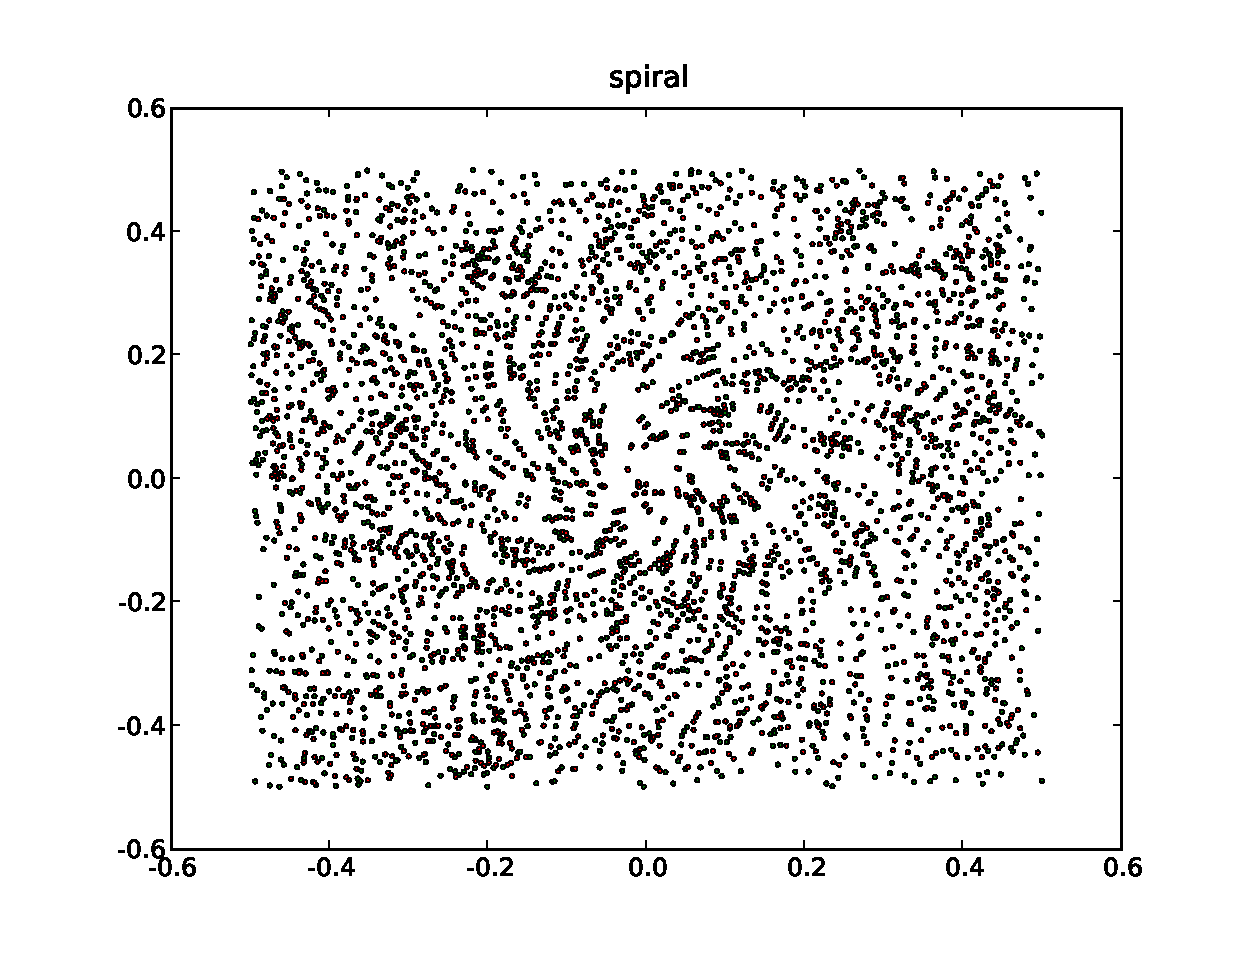
\includegraphics[width=4in]{fig/glass_dots1}\par\end{centering}


\caption{\label{fig:glass_dots1}Glass pattern showing a stable focus}
\end{figure}
\par\end{center}
